%!TEX root = ../[BDSA'21] - Exam Answers.tex

\section{Instructions for Using the \LaTeX\ Skeleton}
\label{sec:skeleton_instructions}

\subsubsection*{On Answers}
For practicality, all answers have been isolated to a single document that contains macros that will automatically place your answer in the correct place of the document.  In this way you will be able to focus purely on the content and not be bothered by the layout and other latex related details.  However, given the special setup, please read the following to ensure you are familiar with the process required to insert them.  Finally, given that you only need to submit the .pdf file, you can edit all files, but this is discouraged.  We verified whether the setup allowed to include the expected answers. 

All macros for the answers are labeled to identify the question and sub element of the question.  For instance, the macro in line one of the example below is used to answer part A of question 1, while the one in line two is designed to fill the gap of the first row column name in the table present in question 13.  
\begin{lstlisting}[language=json,basicstyle=\ttfamily\footnotesize,numbersep=5pt,frame=trBL,framexleftmargin=1.5em]
\def\questionOneAnswerA{} %% Write your answer inside the brackets
\def\questionThirteenAnswerARowOneColumnName{}	% Write your answer inside the brackets
\let\questionOneAnswerA\undefined %% Comment this to enable your answer
\end{lstlisting}

\underline{Important:} some questions (see line three) are followed by a line that removes their definition.  This is necessary to allow the layout of a proper empty answer without polluting the macro you have to use for the answer.  If you decide to answer these questions, which are most of the text based answers, make sure to comment out or remove the line so that your answer will be shown.  In the following, possible type of answers are specified.


\subsubsection*{On Text Answers}
\begin{lstlisting}[language=json,basicstyle=\ttfamily\footnotesize,numbersep=5pt,frame=trBL,framexleftmargin=1.5em]
\def\questionOneAnswerA{} %% Write your answer inside the brackets
\let\questionOneAnswerA\undefined %% Comment this to enable your answer
\end{lstlisting}

These are captured as shown in the listing above.  Your task is first to comment out or delete the redefinition of the macro (line 2) and second to provide your answer between the curly brackets of the macro in line 1.  

The possibilities here are up to your knowledge of \LaTeX.  For instance, you can use specific environments like enumerate, description, or itemize as shown below.  Notice that line 15 is commented out.
\begin{lstlisting}[language=json,basicstyle=\ttfamily\footnotesize,numbersep=5pt,frame=trBL,framexleftmargin=1.5em]
\def\questionOneAnswerA{
\begin{itemize}
	\item my answer point 1
	\item my answer point 2
	\end{itemize}
\begin{enumerate}[I.]
	\item my answer point 1
	\item my answer point 2
	\end{enumerate}
\begin{description}
	\item[point 1] this is why
	\item[point 2] and this is even more
	\end{description}
	} %% Write your answer inside the brackets
% \let\questionOneAnswerA\undefined %% Comment this to enable your answer
\end{lstlisting}
\begin{center}
	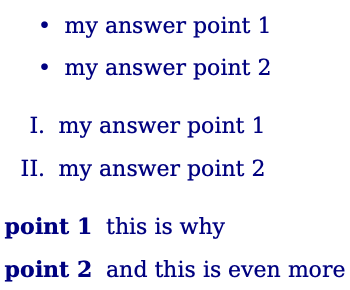
\includegraphics[width=.4\columnwidth]{img/example1}
\end{center}



\subsubsection*{On True/False Answers}
If the question requires a True/False answer, you are expected to write either `True' or `False' (no quotation mark).  As mentioned in the comment, these are case sensitive and will generate a ticked square and an empty square accordingly.  Were you not interested in answering the question, you can leave the macro untouched.  Any input different from either `True' or `False' will result in empty squares.
\begin{lstlisting}[language=json,basicstyle=\ttfamily\footnotesize,numbersep=5pt,frame=trBL,framexleftmargin=1.5em]
\def\questionOneAnswerA{}	% Case sensitive: use either 'True' or 'False'
\end{lstlisting}



\subsubsection*{On Answers Requiring the Checking of Boxes}
If the question requires a check on a box as an answer, you are expected to comment out or delete the wrong one and uncomment or leave as is the correct one.  As mentioned in the comment, the two lines are described: one will produced a checked box, while the other an empty box.  Were you not interested in answering the question, you can leave the macros untouched.  
\begin{lstlisting}[language=json,basicstyle=\ttfamily\footnotesize,numbersep=5pt,frame=trBL,framexleftmargin=1.5em]
\def\questionTwoAnswerARowOneColumnKey{\centerbox}	% not checked
% \def\questionTwoAnswerARowOneColumnKey{\centercheckedbox} % checked
\end{lstlisting}





\subsubsection*{On Answers Requiring Code}
To support an easy approach to inserting code, the template has a dedicated process for code handling.  When facing a question that requires a code snippet as an answer, you will be presented with a macro that contains a reference to a .tex file with the code solution.  The folder and file have already been created, so that you can just open the file and insert the code.  
\begin{lstlisting}[language=json,basicstyle=\ttfamily\footnotesize,numbersep=5pt,frame=trBL,framexleftmargin=1.5em]
\def\questionOneAnswerA{answers/code/q01_answerB} %% edit the content of the file
\end{lstlisting}

Its layout needs to be contain in the lstlisting environment (already included in all files) as shown in the example below, and when compiled will reproduced verbatim the code in the .pdf.
Again, the file is already available for you to edit and, in some cases, will contain some minor code instructions to help guiding you in answering the question.
\begin{lstlisting}[language=json,basicstyle=\ttfamily\footnotesize,numbersep=5pt,frame=trBL,framexleftmargin=1.5em]
%!TEX root = ../../[BDSA'21] - Exam Answers.tex

\begin{lstlisting}
public class Artist
{


}
\end{lstlisting_} % the underscore is included only in this example to avoid conflicts between the environments 
\end{lstlisting}



\subsubsection*{On Answers Requiring Diagrams}
To support an easy approach to inserting diagrams, the template has a dedicated process for handling them.  When facing a question that requires a diagram as an answer, you will be presented with a macro that contains a reference to a file (line 2).  The folder and file have already been created, so that you can just replace the file with yours.  
\begin{lstlisting}[language=json,basicstyle=\ttfamily\footnotesize,numbersep=5pt,frame=trBL,framexleftmargin=1.5em]
\def\questionOneAnswerAwidth{.8} %% If necessary consider adjusting the multiplying factor
\def\questionOneAnswerA{answers/diagrams/q01_answerA} %% link the file containing the diagram
\end{lstlisting}

The file provided with this skeleton is a .png, but the system is tested also for inclusion of .pdf files.  A multiplying factor has also been exposed through a macro so that, in case necessary, you will be able to enlarge or reduce the resulting image.  The solutions have been tested on this setup, and it should not be necessary to modify that factor.

